% Baccalauréat malgache, série C, 2004 : corrigé.
\TCDBacAttribution{C}{2004}
\providecommand{\Milimetre}[2]{%
									\clip #1 rectangle #2;
									\draw [xstep=0.1cm,ystep=0.1cm,opacity=.05,line width=.05] #1 grid #2;
									\draw [xstep=0.5cm,ystep=0.5cm,opacity=0.1,line width=0.1] #1 grid #2;
									\draw [xstep=1.0cm,ystep=1.0cm,opacity=0.2,line width=0.2] #1 grid #2;
									}
\providecommand{\Plan}{(\mathscr{P})}
\providecommand{\dx}{~\mathrm{d}x}
\providecommand{\Re}[1]{\mathrm{Re}\left( #1 \right)}
\providecommand{\Im}[1]{\mathrm{Im}\left( #1 \right)}
\providecommand{\dt}{\mathrm{d}t}
\providecommand{\Ouv}{(O;\vec{u},\vec{v})}
\providecommand{\mes}[2]{\mathrm{mes}\left( \widehat{ \overrightarrow{#1} ; \overrightarrow{#2} } \right)}
\providecommand{\D}{(\mathscr{D})}
\providecommand{\Courbe}{(\mathscr{C})}
\providecommand{\Courben}{(\mathscr{C}_n)}
\providecommand{\CourbeU}{(\mathscr{C}_1)}
\providecommand{\CourbeD}{(\mathscr{C}_2)}
\providecommand{\bary}[1]{\mathrm{bar}\left\lbrace #1 \right\rbrace}
\providecommand{\CourbeT}{(\mathscr{C}_3)}
\providecommand{\congru}[3]{#1 \equi #2 \quad \left[ \mathrm{mod}~#3\right]}
\providecommand{\Angl}[2]{\left( \widehat{ \overrightarrow{#1} , \overrightarrow{#2} } \right)}
%
%%%%%%%%%%%%%%%%%%%%%%%%%%%%%%%%%%%%%%%%%%%%%%%%%%%%%%%%%%%%%%%%%%%%%%%%%%%%%%%%%%%%%%%%%%%%%%%%%%%%%%%%%%%%%%%%%%%%%%%%%%%%%%%%
\noindent \underline{\textsc{\textbf{Exercice}}} (4 points) 
	\begin{description}
		\item[I. ]
			\begin{enumerate}
				\item \begin{itemize}
							\item \vln{Probabilit\'e de $A$ :}
								$P(A) = \frac{\text{Nombre de faces num\'erot\'ees }0}{\text{Nombre total de faces}} = \frac{4}{6}$.
								Donc \ansbox{$P(A) = \frac{2}{3}$.}
							\item \vln{Probabilit\'e de $B$ :}
								$P(B) = \frac{\text{Nombre de faces num\'erot\'ees }1}{\text{Nombre total de faces}} = \frac{2}{6}$.
								Donc \ansbox{$P(B) = \frac{1}{3}$.}
						\end{itemize}
				\item Cette exp\'erience suit un sch\'ema de Bernoulli.
						Si on d\'efinit le << succ\`es >> comme l'obtention d'une face num\'erot\'ee $0$,
						on a une loi de Bernoulli de param\`etres $(5 ; \frac{2}{3})$.
						\begin{itemize}
							\item \vln{Probabilit\'e de $C$ :}
								$
									P(C) = \text{Probabilit\'e d'avoir 1 << succ\`es >>}
										= \Comb{5}{1} \cdot \left( \frac{2}{3} \right)^1 \cdot \left( \frac{1}{3} \right)^4
									 	= 5 \cdot \frac{2}{3} \cdot \frac{1}{81}
								$
								donc \ansbox{$P(C) = \frac{10}{243}$.}
							\item \vln{Probabilit\'e de $D$ :}
								$
									P(D) = \text{Probabilit\'e d'avoir 0 << succ\`es >>}
										= \Comb{5}{0} \cdot \left( \frac{2}{3} \right)^0 \cdot \left( \frac{1}{3} \right)^5
									 	= 1 \cdot \frac{1}{243} \cdot 1
								$
								donc \ansbox{$P(D) = \frac{1}{243}$.}
							\item \vln{Probabilit\'e de $E$ :}
								$E$ : Avoir au moins un \emph{succ\`es}.
								Par cons\'equent, $\bar{E}$ : Avoir 5 \'echecs : $D$.
								Donc $P(E) = 1 - P(\bar{E}) = 1 - P(D) = 1 - \frac{1}{243}$.
								Ainsi, \ansbox{$P(E) = \frac{242}{243}$.}
						\end{itemize}
			\end{enumerate}
		\item[II. ]
			\begin{enumerate}
				\item \begin{enumerate}
								\item \vln{Conversion de $x$ en base 10 :}
								$x = 1\cdot 2^4 + 0 \cdot 2^3 + 1 \cdot 2^2 + 0 \cdot 2^1 + 1 \cdot 2^0 = 21$.
								Donc \ansbox{$x = 21$}.
								\item \vln{Conversion de $y$ en binaire :}
								\begin{center}
									\begin{tikzpicture}[>=stealth,x=.4cm,y=.4cm]
									\draw (1,2)-- (3,2);
									\draw (1,3)-- (1,0);
									\draw (3,1)-- (5,1);
									\draw (3,2)-- (3,-1);
									\draw (5,0)-- (7,0);
									\draw (5,1)-- (5,-2);
									\draw (7,-1)-- (9,-1);
									\draw (7,0)-- (7,-3);
									\draw (0,2.5) node  {23};
									\draw (2,2.5) node  {2};
									\draw (4,1.5) node  {2};
									\draw (6,0.5) node  {2};
									\draw (8,-0.5) node  {2};
									\draw (2,1.5) node  {11};
									\draw (0,1.5) node  {\underline{22}};
									\draw (0,0.5) node  {\phantom{1}1};
									\draw (4,0.5) node  {5};
									\draw (2,0.5) node  {\underline{10}};
									\draw (2,-0.5) node  {\phantom{1}1};
									\draw (6,-0.5) node  {2};
									\draw (4,-0.5) node  {\underline{4}};
									\draw (4,-1.5) node  {1};
									\draw (8,-1.5) node  {1};
									\draw (6,-1.5) node  {\underline{2}};
									\draw (6,-2.5) node  {0};
									\draw [->,line width = .75ex, opacity=.35,color=loko3,smooth,rounded corners=1ex] 
										(8,-2) -- (6,-3.25) -- (-0.25,0.25) ;
									\end{tikzpicture}
								\end{center}
								Donc \ansbox{$ y = (\overline{10111})_2$.}
						\end{enumerate}
				\item \begin{enumerate}
							\item \vln{Table de multiplication de $\mathbb{Z}/2\mathbb{Z}$ :}
										\[
											\begin{array}{|c|c|c|}
																	\hline
												\times 	& \bar{0} & \bar{1} \\\hline
												\bar{0}	& \bar{0} & \bar{0} \\\hline
												\bar{1}	& \bar{0} & \bar{1} \\\hline
											\end{array}
												\qquad	\qquad	\qquad
											\begin{array}{|c|c|c|}
																	\hline
													 +		& \bar{0} & \bar{1} \\\hline
												\bar{0}	& \bar{0} & \bar{1} \\\hline
												\bar{1}	& \bar{1} & \bar{0} \\\hline
											\end{array}
										\]
							\item \vln{R\'esolution dans $\mathbb{Z}/2\mathbb{Z}$ de $ x^2 + x + \bar{2} = \bar{0} $ :}
										\[
											x^2 + x + \bar{2} = \bar{0}	\iff x^2 + x = \bar{0}
										\]
										\begin{description}
											\item[Si $x = \bar{0}$ : ] $\bar{0}^2 + \bar{0} = \bar{0}$,
											\item[Si $x = \bar{1}$ : ] $\bar{1}^2 + \bar{1} = \bar{1} + \bar{1} = \bar{0}$.
										\end{description}
									Donc \ansbox{l'ensemble des solutions est $\left\lbrace \bar{0}\ ;\ \bar{1} \right\rbrace$.}
							\item \vln{R\'esolution dans $\mathbb{Z}/2\mathbb{Z} \times \mathbb{Z}/2\mathbb{Z}$ du syst\`eme 
									$\begin{multiform} \bar{2}x+y = \bar{0} \\ x+\bar{3}y = \bar{0} \end{multiform}$ :}
									Comme $\bar{2} = \bar{0}$ et $\bar{3} = \bar{1}$, ce syst\`eme est \'equivalent \`a 
									$\begin{multiform}y = \bar{0}\\ x + y = \bar{0}\end{multiform}$.
									Comme $y=\bar{0}$, $x + \bar{0}= \bar{0}$ donc $x = \bar{0}$.
									Ainsi, \ansbox{$(x,y) = \left( \bar{0} , \bar{0} \right)$}.
						\end{enumerate}
			\end{enumerate}
	\end{description}
%%%%%%%%%%%%%%%%%%%%%%%%%%%%%%%%%%%%%%%%%%%%%%%%%%%%%%%%%%%%%%%%%%%%%%%%%%%%%%%%%%%%%%%%%%%%%%%%%%%%%%%%%%%%%%%%%%%%%%%%%%%%%%%%
\noindent \underline{\textsc{\textbf{PROBLEME I}}} (7 points) \newline
	\begin{description}
		\item[Partie A]
			\begin{enumerate}
				\item \begin{enumerate}
					\item \vln{D\'eterminons $G$ :}
						Comme $G = \bary{(A,-1);(B,1);(C,1)}$ alors 
						\begin{align*}
						-\overrightarrow{GA}+\overrightarrow{GB}+\overrightarrow{GC} & = \vec{0}	\\
						-\overrightarrow{GA}+\overrightarrow{GA}+\overrightarrow{AB}+\overrightarrow{GA}+\overrightarrow{AC}&=\vec{0}	\\
						\overrightarrow{AB}+\overrightarrow{AC}=\overrightarrow{AG}	.
						\end{align*}
						Ainsi, \ansbox{$\overrightarrow{AG}=\overrightarrow{AB}+\overrightarrow{AC}$.}
							
							\vln{Construction de $G$ :}
								\begin{figure}[h!]
									\centering
									\resizebox{\linewidth}{!}{%
									\begin{tikzpicture}[line cap=round,line join=round,>=triangle 45,x=1.0cm,y=1.0cm]
									\Milimetre{(-1,-3)}{(13,9)}
									\coordinate (A) at (0,0);
									\coordinate (B) at (8,0);
									\coordinate (C) at (0,4);
									\coordinate (I) at (4,0);
									\coordinate (J) at (0,2);
									\coordinate (E) at (4,2);
									\coordinate (G) at (8,4);
									\coordinate (K) at (4,4);
									\draw [->] (A) -- (B);
									\draw [->] (A) -- (C);
									\draw [->] (A) -- (G);
									\draw (0,0)-- (8,0);
									\draw (8,0)-- (0,4);
									\draw (0,4)-- (0,0);
										\fill [color=black] (A) circle (1.5pt) node[above left] {$A$};
										\fill [color=black] (B) circle (1.5pt) node[above right] {$B$};
										\fill [color=black] (C) circle (1.5pt) node[above left] {$C$};
										\fill  (I) circle (1.5pt) node[above right] {$I$};
										\fill  (J) circle (1.5pt) node[above right] {$J$};
										\fill  (E) circle (1.5pt) node[below] {$E$};
										\fill  (K) circle (1.5pt) node[above] {$K$};
										\draw [color=loko3!75!black, ultra thick] (G) circle (1.5pt) node[below right] {$D$};
										\fill [color=loko1] (G) circle (1.5pt) node[above right] {$G$};
									\draw [color=loko5, dashed] (E) circle (4.47213595499958);
									\draw [color=loko1] (G) circle (4.47213595499958) (3.5,5.5) node {$(\mathscr{C})$};
									\end{tikzpicture}%
									}
							\end{figure}
					\item \vln{Expression de $\overrightarrow{AG}$ en fonction de $\overrightarrow{AE}$ :}
								Comme $E$ est milieu de $[BC]$, alors 
								$\overrightarrow{EB}+\overrightarrow{EC}=\vec{0}$.
								\begin{align*}
									\overrightarrow{EB}+\overrightarrow{EC} & = \vec{0}		\\
									\overrightarrow{EA}+\overrightarrow{AB}+\overrightarrow{EA}+\overrightarrow{AC} & = \vec{0}		\\
									\overrightarrow{AB}+\overrightarrow{AC} + 2 \overrightarrow{EA}	& = \vec{0}	\\
									\overrightarrow{AG} & = -2\overrightarrow{EA}		.
								\end{align*}
								Ainsi, \ansbox{$\overrightarrow{AG} = 2 \overrightarrow{AE}$.}
							
							\vln{Calcul de $AG$ :}
								Comme $ABGC$ est un rectangle, alors $AG = BC$.
								Le triangle $ABC$ \'etant rectangle en $A$, d'apr\`es le th\'eor\`eme de Pythagore :
									$BC^2 = AB^2 + AC^2$.
								Ainsi, $AG = BC = \sqrt{AB^2 + AC^2} = \sqrt{8^2 + 4^2}$, d'o\`u \ansbox{$AG = 4 \sqrt{5}$}.
					\item \vln{Montrons que $E$ est le centre du cercle circonscrit au triangle $ABC$ :}
								Comme $ABCG$ est un rectangle et que $E$ est l'intersection des ses diagonales,
								\ansbox{le cercle de centre $E$ et passant par $A$ passe aussi par $B$, $C$} et $G$.
								Ce cercle est le cercle circonscrit au triangle $ABC$.
					\item \vln{Construction du point $D$ :}
								Les points $D$ et $G$ sont confondus.
							
							\vln{Deux isom\'etries qui laissent globalement invariant le rectangle $(ABDC)$ :} \vspace{-1\baselineskip}
								\begin{itemize}
									\item Rotation de centre $E$ et d'angle $\pi$ : 
										les images de $A$, $B$, $D$ et $C$ par cette rotation sont $D$, $C$, $A$ et $B$.
									\item Sym\'etrie orthogonale d'axe $(EI)$ :
										les images de $A$, $B$, $D$ et $C$ par cette sym\'etrie sont $B$, $A$, $C$ et $D$.
								\end{itemize}
								{\color{loko3}
								Il y aussi :
								\begin{itemize}
									\item Sym\'etrie orthogonale d'axe $(EJ)$ :
										les images de $A$, $B$, $D$ et $C$ par cette sym\'etrie sont $C$, $D$, $B$ et $A$.
									\item Application identit\'e :
										tout sous-ensemble est laiss\'e invariant.
								\end{itemize}
								}
						\item \vln{D\'eterminons $(\mathscr{C})$ :}
							Soit $\varphi$ la fonction scalaire de Leibniz associ\'ee au syst\`eme
							\[
							\{(A,-1);(B,1);(C,1)\}.
							\]
							Comme $ABGC$ est un rectangle, $GA=BC$ ; comme le triangle $BGC$ est rectangle en $G$,
							on a donc $GA^2=GB^2+GC^2$.
						Par cons\'equent, $\varphi(G) = -GA^2 + GB^2 + GC^2 = 0$.
						On sait que
						\[
							\varphi(M)	 = (-1+1+1) \cdot MG^2 + \varphi(G)
											 = MG^2										
						\]
						\begin{align*}
								(\mathscr{C})	& = \left\{ M \in \Plan \mid -MA^2 + MB^2 + MC^2 = 20 \right\}					\\
												& = \left\{ M \in \Plan \mid MG^2 = \left( 2\sqrt{5} \right)^2 \right\}		.
						\end{align*}
						Donc $(\mathscr{C})$ est le cercle de centre $G$ et de rayon $2\sqrt{5}$.

						Le cercle \ansbox{$(\mathscr{C})$ a pour centre $G$ et passe par $E$.}
						
						\vln{Construction de $(\mathscr{C})$ :} voir Figure.
					\end{enumerate}
				\item \vln{Montrons que pour tout $M$ du plan contenant $A$, $B$ et $C$, 
						$-\frac{3}{2}\overrightarrow{MA}+\frac{1}{2}\overrightarrow{MB}+\overrightarrow{MC}$
						est un vecteur fixe $\overrightarrow{W}$ que l'on determinera :}
							\begin{align*}
								-\frac{3}{2}\overrightarrow{MA}+\frac{1}{2}\overrightarrow{MB}+\overrightarrow{MC} & = 
								-\frac{3}{2}\overrightarrow{MA}
									+\frac{1}{2}\overrightarrow{MA}
										+\frac{1}{2}\overrightarrow{AB}
											+\overrightarrow{MA}+\overrightarrow{AC}	\\	& =
								\frac{1}{2} \overrightarrow{AB} + \overrightarrow{AC} .
							\end{align*}
							Donc \ansbox{$-\frac{3}{2}\overrightarrow{MA}+\frac{1}{2}\overrightarrow{MB}+\overrightarrow{MC}$
							est toujours \'egal \`a $\overrightarrow{W} = \frac{1}{2} \overrightarrow{AB} + \overrightarrow{AC}$.}
						
						\vln{Construction de $K$ :}
							$\overrightarrow{W} = \overrightarrow{AK} = \frac{1}{2} \overrightarrow{AB} + \overrightarrow{AC}$.
							(voir Figure)
			\end{enumerate}
				\item[Partie B]
					\begin{enumerate}
						\item \vln{D\'eterminons $z_A$, $z_B$, $z_C$ et $z_I$ :}
							\begin{itemize}
								\item \ansbox{$z_A = 0$} car $A$ est l'origine.
								\item \ansbox{$z_B = 8$} car 
									$\vec{u} = \frac{1}{8} \cdot \overrightarrow{AB} \Rightarrow \overrightarrow{AB} = 8 \vec{u}$.
								\item \ansbox{$z_C = 4i$} car 
									$\vec{v} = \frac{1}{4} \cdot \overrightarrow{AC} \Rightarrow \overrightarrow{AC} = 4 \vec{v}$.
								\item \ansbox{$z_I = 4$} car 
									$\overrightarrow{AI} = \frac{1}{2} \overrightarrow{AB} \Rightarrow z_I = \frac{1}{2} z_B$.
							\end{itemize}
						\item \begin{enumerate}
									\item \vln{D\'eterminons l'expression complexes de $S_1$ :}
												Soit $z' = a\, z + b$ l'expression complexe de $S_1$.
												Comme 
												$\begin{multiform}S_1(C)=C\\ S_1(I)=A\end{multiform}$, 
												alors
												\begin{align*}
												a	& = \frac{z_C - z_A}{z_C - z_I}		& z_C & = a \, z_C + b 		\\
													& = \frac{4i}{4i - 4}						& b 	& = z_c ( 1 - a)		\\
													& = \frac{i\,(-i-1)}{(i-1)\,(-i-1)}	&  		& = 4i\left(1-\frac{1}{2}+\frac{i}{2}\right) \\
													& = \frac{1-i}{1+1}						&   	& = 4i\left(\frac{1}{2}+\frac{i}{2}\right)	\\
													& = \frac{1}{2} - \frac{i}{2}			&  		& = -2 + 2i 				.
												\end{align*}
												Ainsi, \ansbox{$ S_1 : z' = \frac{1-i}{2} \; z - 2+ 2i $.}
												
											\vln{D\'eterminons l'expression complexes de $S_2$ :}
												Soit $z' = a\, z + b$ l'expression complexe de $S_2$ ($a$ et $b$ ne sont plus ceux de $S_1$).
												Comme 
												$\begin{multiform}S_2(I)=I\\ S_2(A)=C\end{multiform}$, 
												alors
												\begin{align*}
												a	& = \frac{z_I - z_C}{z_I - z_A}		& z_I & = a \, z_I + b 		\\
													& = \frac{4-4i}{4}							& b 	& = z_I ( 1 - a)		\\
													& = 1-i										&  		& = 4 (1-1+i) = 4i		.
												\end{align*}
												Ainsi, \ansbox{$ S_2 : z' = (1-i) \; z +4i $.}
									\item \vln{\'El\'ements caract\'eristiques de $S_1$ :}\vspace{-1\baselineskip}
												\begin{description}
													\item[Rapport :] 
														$\left|\frac{1-i}{2}\right| = \frac{1}{2}\sqrt{1^2 + 1^2} = \frac{\sqrt{2}}{2}$.
													\item[Angle $\theta_1$ :]
														$\frac{1-i}{2}=\frac{\sqrt{2}}{2}\left(\frac{\sqrt{2}}{2}-\frac{\sqrt{2}}{2}\right)i$
														donc 
														$\left|
														\begin{matrix}
															\cos \theta_1 = \frac{\sqrt{2}}{2}	\\
															\sin \theta_1 = -\frac{\sqrt{2}}{2}
														\end{matrix}
														\right\rbrace 
														\Rightarrow
														\theta_1 = -\frac{\pi}{4}.
														$
													\item[Centre :] Comme $S_1(C) = C$ alors $C$ est le centre.
												\end{description}
												Donc 
												\ansbox{
												$S_1$ a pour centre $C$, pour rapport $\frac{\sqrt{2}}{2}$ et pour angle $-\frac{\pi}{4}$
												.}
												
											\vln{\'El\'ements caract\'eristiques de $S_2$ :}\vspace{-1\baselineskip}
												\begin{description}
													\item[Rapport :] $|1-i| = \sqrt{2}$.
													\item[Angle $\theta_2$:] 
														$1-i = \sqrt{2} \left( \frac{\sqrt{2}}{2} - \frac{\sqrt{2}}{2} i\right)$ donc
														$\left|
															\begin{matrix}
																\cos \theta_2 = \frac{\sqrt{2}}{2}	\\
																\sin \theta_2 = -\frac{\sqrt{2}}{2}	
															\end{matrix}
														\right\rbrace
														\Rightarrow
														\theta_2 = -\frac{\pi}{4}.
														$
													\item[Centre :] Comme $S_2(I) = I$ alors $I$ est le centre de $S_2$.
												\end{description}
												Donc 
												\ansbox{
												$S_2$ a pour centre $I$, pour rapport $\sqrt{2}$ et pour angle $-\frac{\pi}{4}$
												.}
								\end{enumerate}
						\item 
								\begin{enumerate}
									\item \vln{Image de $I$ par $R$ :}
												$R(I) = S_2 \left( S_1(I) \right) = S_2 (A) = C$ donc \ansbox{$R(I) = C$}.
									\item \vln{Expression complexe de $R$ :}
												$
													\left.
														\begin{matrix}
															S_1 : z' = \frac{1-i}{2}z -2 + 2i \\
															S_2 : z' = (1-i) z + 4 i
														\end{matrix}
													\right\rbrace
													\Rightarrow
														\begin{array}[t]{l@{\ }l}
															R : z'	& = (1-i) \left[ \frac{1-i}{2}z -2 + 2i \right] + 4i		\\
																	& = \frac{(1-i)^2}{2} z -2 (1-i) (1-i) + 4i					.
														\end{array}
												$
												
											Par cons\'equent, l'expression complexe de $R$ est donn\'ee par
												\ansbox{$z' = -i \; z + 8i$.}
									\item \vln{\'El\'ements g\'eom\'etriques de $R$ :}
												\begin{description}
													\item[Angle $\theta$ :] $\Arg{-i} = -\frac{\pi}{2}$.
													\item[Rapport :] $|-i| = 1$, donc $R$ est juste une rotation.
													\item[Affixe $z_\Omega$ du centre :]
														$z_\Omega = \frac{8i}{1-(-i)} = \frac{8i \; (1-i)}{(1+i)\;(1-i)} = 4 + 4i$
														donc le centre est $K$.
												\end{description}
												Ainsi, \ansbox{$R$ est la rotation de centre $K$ et d'angle $-\frac{\pi}{2}$.}
											
								\end{enumerate}
					\item \vln{Caract\'erisation de $g$ : }
									La transformation $g$ est la similitude plane directe de centre $C$,
									de rapport $\frac{1}{\frac{\sqrt{2}}{2}}=\sqrt{2}$ et d'angle $\frac{\pi}{4}$.
									
									\vln{Expression complexe de $g$ :}
										Soit $z'=\alpha z+\beta$ l'expression complexe de $g$.
										On a alors
										\[
										\left.
											\begin{array}{r}
												|\alpha| = \sqrt{2}				\\
												\Arg{\alpha} = \frac{\pi}{4}	
											\end{array}
										\right\rbrace
										\Rightarrow
										\begin{array}[t]{l@{\ }l}
												\alpha	& 	= \sqrt{2} \; \left( \cos \frac{\pi}{4} + i \sin \frac{\pi}{4} \right)		\\
														& 	= \sqrt{2} \; \left( \frac{\sqrt{2}}{2} + i \frac{\sqrt{2}}{2} \right)		
															= 1 + i.
										\end{array}
										\]
									
										Comme $C$ est invariant par $g$,
										\[
										\begin{aligned}
										z_C&=\alpha z_C+\beta,\\
										4i&=(1+i)4i+\beta,
										\end{aligned}
										\qquad\text{d'o\`u}\qquad \beta=4.
										\]
										Par cons\'equent, $g$ a pour expression complexe $z'=(1+i)z+4$.
					\end{enumerate}
	\end{description}
%%%%%%%%%%%%%%%%%%%%%%%%%%%%%%%%%%%%%%%%%%%%%%%%%%%%%%%%%%%%%%%%%%%%%%%%%%%%%%%%%%%%%%%%%%%%%%%%%%%%%%%%%%%%%%%%%%%%%%%%%%%%%%%%
\noindent \underline{\textsc{\textbf{PROBLEME II}}} (9 points) \newline
	\begin{description}
		\item[Partie A]
			\begin{enumerate}
				\item \vln{Calcul de $I_1$ :}
							\[
								I_1 = \int_{1}^{e} f_1 (x) \dx = \int_{1}^{e} x \cdot \ln x \dx .
							\]
							\textbf{Int\'egrons par partie :} 
							Posons $u = \ln x $ et $v' = x$, on a $u' = \frac{1}{x}$ et $v = \frac{x^2}{2}$.
							\begin{align*}
								I_1	& = \left[ \frac{x^2}{2} \ln x \right]_{1}^{e} - \int_{1}^{e} \frac{x^2}{2} \cdot \frac{1}{x} \dx	
									  = \frac{\expo{2}}{2} - \frac{1}{2} \int_{1}^{e} x \dx \\
									& = \frac{\expo{2}}{2} - \frac{1}{2} \left[ \frac{x^2}{2} \right]_{1}^{e}	
									  = \frac{\expo{2}}{2} - \frac{1}{2} \left[ \frac{\expo{2}}{2} - \frac{1}{2} \right] 
									  = \frac{\expo{2} + 1}{4} .
							\end{align*}
							Ainsi, \ansbox{$I_1 = \frac{\expo{2} + 1}{4}$}.
				\item 
					\begin{enumerate}
						\item \vln{Calcul $I_2$ :}
							$I_2 = \int_{1}^{e} x \; (\ln x)^2 \dx$.
							
							Posons $u' = x$ et $v = (\ln x)^2$, on a $u = \frac{x^2}{2}$ et $v' = 2 \frac{1}{x} \ln x$.
							\begin{align*}
								I_2	& = \left[ \frac{(x \ln x)^2}{2} \right]_{1}^{e} - \int_{1}^{e} x \ln x \dx 
									  = \frac{\expo{2}}{2} - \frac{\expo{2}+1}{4} .
							\end{align*}
							Ainsi, \ansbox{$I_2 = \frac{\expo{2}-1}{4}$}.
						\item \vln{Expression de $I_{n+1}$ en fonction de $I_n$ :}
							Int\'egrons par partie :
							$I_{n+1} = \int_{1}^{e} x (\ln x)^{n+1} \dx$.
							
							Posons $u	= (\ln x)^{n+1}$ et $v'	= x $, on a $u'	= (n+1) \frac{1}{x} (\ln x)^n$ et $v	= \frac{x^2}{2}$.
							\begin{align*}
								I_{n+1}	& = \left[\frac{x^2}{2}(\ln x)^{n+1}\right]_{1}^{e}-\frac{n+1}{2}\int_{1}^{e}x(\ln x)^n\dx	
							\end{align*}
							Donc \ansbox{$\displaystyle{ I_{n+1} = \frac{\expo{2}}{2} - \frac{n+1}{2} I_{n} }$}.
						\item \vln{D\'eduction de $I_3$ :}
							\[
								I_3		= \frac{\expo{2}}{2} - \frac{2 + 1}{2} I_2 
										= \frac{\expo{2}}{2} - \frac{3}{2} \frac{\expo{2} - 1}{4}
										= \frac{4 \expo{2}}{8} - \frac{3 \expo{2} - 3}{8}
							\]
							donc \ansbox{$I_3 = \frac{\expo{2} + 3}{8}$}.
					\end{enumerate}
			\end{enumerate}
		\item[Partie B]
			\begin{description}
				\item[I. ]
					\begin{enumerate}
						\item \begin{enumerate}
									\item \vln{Montrons que $f_n$ est continue en $0$ :}
										\begin{align*}
											\lim_{x\rightarrow 0^+} f_n (x) 
												& = \lim_{x\rightarrow 0^+} x (\ln x)^n 	\\
										\intertext{Posons $t = x^{\frac{1}{n}}$, on a $x = t^n$ et
												 $\xymatrix@1{ t\ar[r]_{x\rightarrow 0^+} & 0^+}$}
											\lim_{x\rightarrow 0^+} f_n (x) 
												& = \lim_{t\rightarrow 0^+} t^n (\ln t^n)^n
											  = \lim_{t\rightarrow 0^+} n^n (t \ln t)^n 			.
										\end{align*}
										Comme $\xymatrix@1{ (t \ln t) \ar[r]_-{t\rightarrow 0^+} & 0}$,
										$\displaystyle{\lim_{x\rightarrow 0^+} f_n (x) = 0 = f_n (0)}$.
										On d\'eduit que \ansbox{$f_n$ est continue en $0$}.
									\item \vln{D\'erivabilit\'e de $f_n$ en $0$ :}
										\[
											\lim_{x\rightarrow 0^+} \frac{f_n (x) - f_n (0)}{x - 0}			
												= \lim_{x\rightarrow 0^+} \frac{x \; (\ln x)^n}{x}			
												= \lim_{x\rightarrow 0^+} (\ln x)^n .
										\]
										\begin{description}
											\item[Si $n$ est pair :] $ \lim_{x\rightarrow 0^+} (\ln x)^n = +\infty$.
											\item[Si $n$ est impair :] $ \lim_{x\rightarrow 0^+} (\ln x)^n = -\infty$.
										\end{description}
										On d\'eduit que \ansbox{$f_n$ n'est pas d\'erivable en $0$}.
									\item \vln{Tangente \`a $\Courben$ au point d'affixe $x_0 = 0$ :}
										\ansbox{La tangente \`a $\Courben$ au point d’abscisse $x_0 = 0$ est verticale.}
								\end{enumerate}
						\item \vln{Montrons que l'\'equation $f_{n+1} (x) - f_n (x) = 0$ 
								admet trois solutions dans l'intervalle $[0;+\infty[$ :}\vspace{-1\baselineskip}
									\begin{align*}
										f_{n+1} (x) - f_{n} (x)	&	= x (\ln x)^{n+1} - x (\ln x)^{n}				\\
																		&	= x \cdot (\ln x)^{n} \cdot (\ln x - 1)		\\
										f_{n+1} (x) - f_{n} (x)	= 0 
																		& \iff x = 0 \text{, } \ln x = 0 \text{ ou } \ln x - 1 = 0		\\
																		& \iff x = 0 \text{, } x = \expo{0} \text{ ou } \ln x = 1 .
									\end{align*}
								Ainsi, l'\'equation $f_{n+1}(x)-f_n(x)=0$ admet trois solutions :
								\par\noindent\ansbox{$0$, $1$ et $e$.}
						\item \vln{D\'eduction que toutes les courbes $\Courben$ passent par 3 points fixes 
										dont on pr\'ecisera les coordonn\'ees :}
								Comme $f_{n+1}(x)-f_n(x)=0$ est \'equivalent \`a $f_{n+1}(x)=f_n(x)$,
								toutes les courbes passent par les m\^emes points :
								\par\noindent\ansbox{$(0,0)$, $(1,0)$ et $(e,e)$.}
					\end{enumerate}
				\item[II. ]
					\begin{enumerate}
						\item \vln{$\displaystyle{\lim_{x \rightarrow +\infty} f_n (x) }$ :}
							Comme $\displaystyle{\lim_{x\rightarrow +\infty} \ln x = +\infty}$
							alors $\displaystyle{\lim_{x\rightarrow +\infty} (\ln x)^n = +\infty}$.
							\[
								\left.
									\begin{array}{r}
										\displaystyle{\lim_{x\rightarrow +\infty} x = +\infty		}			\\
										\displaystyle{\lim_{x\rightarrow +\infty} (\ln x)^n = +\infty}
									\end{array}
								\right\rbrace
								\Rightarrow
								\lim_{x\rightarrow +\infty} x (\ln x)^n = +\infty	
							\]
								Ainsi,
								\par\noindent\ansbox{$\displaystyle\lim_{x\rightarrow +\infty} f_n(x)=+\infty$.}
						\item \vln{Montrons que pour tout $x > 0$ : $f_n ' (x) = [n + \ln x] [\ln x]^{n-1}$ :}
							Posons $u = x$ et $v = (\ln x)^n$ ; on a $u' = 1$ et $v' = n \frac{1}{x} (\ln x)^{n-1}$.
							Comme $f_{n} (x) = u \cdot v$ alors 
							\[
								f_n ' (x)	= (\ln x)^n + \frac{n (\ln x)^{n-1}}{\not x} \cdot \not x			
											= \left( (\ln x)^{n-1} \right) \cdot \left( \ln x + n \right)		.
							\]
								Ainsi,
								\par\noindent\ansbox{$f_n'(x)=(n+\ln x)(\ln x)^{n-1}$.}
						\item \textbf{Pour $n$ impair :} 
							\begin{enumerate}
								\item \vln{Montrons que $f_n '(x)$ et $[n + \ln x]$ sont de m\^eme signe :}
									Si $n$ est impair alors $n-1$ est pair et donc $\left[ \ln x \right]^{n-1} \geq 0$.
									Il suit que
									\par\noindent\ansbox{$f_n'(x)$ et $n+\ln x$ sont de m\^eme signe.}
								\item \vln{Tableau de variation de $f_n$ :}
											$f'_n(x) = 0 \iff n + \ln x = 0 \iff \ln x = -n \iff x = \expo{-n}$.
											\begin{figure}[h!]
											\centering
												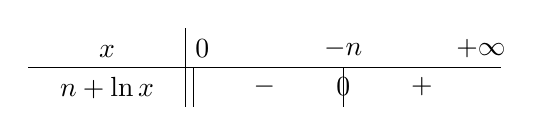
\begin{tikzpicture}
													\draw (-2,0) -- (4,0) 
															(0,.5) -- (0,-.5)
															(0.1,0) -- (0.1,-.5)
															(2,0) -- (2,-.5);
													\draw (-1,0) node[above] {$x$}
															(0,0) node[above right] {$0$}
															(2,0) node[above] {$\expo{-n}$}
															(2,0) node[below] {$0$}
															(3.75,0) node[above] {$+\infty$}
															(-1,0) node[below] {$n + \ln x$}
															(1,0) node[below] {$-$}
															(3,0) node[below] {$+$};
												\end{tikzpicture}
											\end{figure}
											%
											$
											f_n \left( \expo{-n} \right)	= \expo{-n} \left( \ln \expo{-n} \right)^n
																					= \frac{1}{\expo{n}} \left( -n \right)^n
																					= \left(\frac{1}{e}\right)^n \cdot \left( -n \right)^n .
											$
											%
											\begin{figure}[h!]
											\centering
												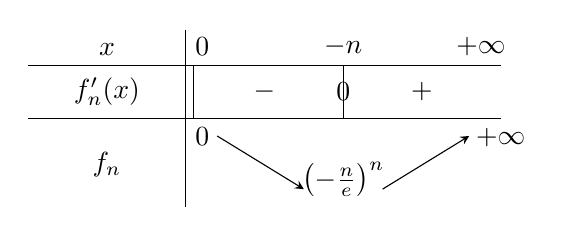
\begin{tikzpicture}[>=stealth,y=.9cm]
													\draw (-2,0) -- (4,0) 
															(-2,-.75) -- (4,-.75) 
															(0,.5) -- (0,-2)
															(0.1,0) -- (0.1,-.75)
															(2,0) -- (2,-.75);
													\draw (-1,0) node[above] {$x$}
															(0,0) node[above right] {$0$}
															(2,0) node[above] {$\expo{-n}$}
															(2,-.375) node[ ] {$0$}
															(3.75,0) node[above] {$+\infty$}
															(-1,-.375) node[ ] {$f'_n(x)$}
															(1,-.375) node[ ] {$-$}
															(3,-.375) node[ ] {$+$}
															(-1,-1.4) node[ ] {$f_n$}
 ;
													\draw [->]	(0.4,-1) -- (1.5,-1.75);
													\draw [->]	(2.5,-1.75) -- (3.6,-1);
													\draw (0,-.75) node[below right] {$0$}
															(2,-2) node[above] {$\left( -\frac{n}{e} \right)^n$}
															(4,-.75) node[below] {$+\infty$}
 ;
												\end{tikzpicture}
											\end{figure}
											
										\vln{Tableau de variation de $f_3$ :}\vspace{-1\baselineskip}
											\begin{figure}[h!]
											\centering
												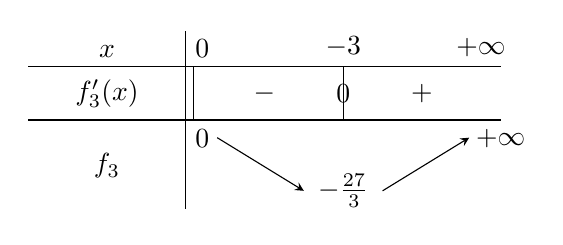
\begin{tikzpicture}[>=stealth,y=.9cm]
													\draw (-2,0) -- (4,0) 
															(-2,-.75) -- (4,-.75) 
															(0,.5) -- (0,-2)
															(0.1,0) -- (0.1,-.75)
															(2,0) -- (2,-.75);
													\draw (-1,0) node[above] {$x$}
															(0,0) node[above right] {$0$}
															(2,0) node[above] {$\expo{-3}$}
															(2,-.375) node[ ] {$0$}
															(3.75,0) node[above] {$+\infty$}
															(-1,-.375) node[ ] {$f'_3(x)$}
															(1,-.375) node[ ] {$-$}
															(3,-.375) node[ ] {$+$}
															(-1,-1.4) node[ ] {$f_3$}
 ;
													\draw [->]	(0.4,-1) -- (1.5,-1.75);
													\draw [->]	(2.5,-1.75) -- (3.6,-1);
													\draw (0,-.75) node[below right] {$0$}
															(2,-1.75) node[] {$-\frac{27}{\expo{3}}$}
															(4,-.75) node[below] {$+\infty$}
 ;
												\end{tikzpicture}
											\end{figure}

							\end{enumerate}
						\item \textbf{Pour $n$ pair :}
							\begin{enumerate}
								\item \vln{Montrons que :}
									On sait que $f'_n(x) = (n + \ln x) \cdot (\ln x)^{n-1}$.
									Comme $n$ est pair, $n-1$ est impair ;
									par cons\'equent $(\ln x)^{n-1}$ et $\ln x$ ont m\^eme signe.
									\begin{figure}[H]
									\centering
										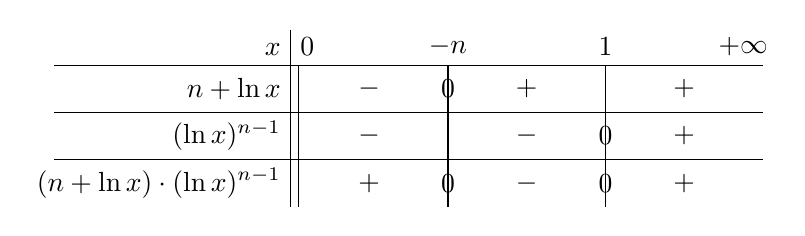
\begin{tikzpicture}[x=1cm,y=.6cm]
											\draw (-3,0) -- (6,0) 
													(-3,-1) -- (6,-1) 
													(-3,-2) -- (6,-2) 
													(0,.75) -- (0,-3)
													(0.1,0) -- (0.1,-3)
													(2,0) -- (2,-3)
													(4,0) -- (4,-3);
											\draw (0,0) node[above left] {$x$}
													(0,0) node[above right] {$0$}
													(2,0) node[above] {$\expo{-n}$}
													(4,0) node[above] {$1$}
													(5.75,0) node[above] {$+\infty$};
											\draw (0,-.5) node[left] {$n + \ln x$}
													(1,-.5) node[] {$-$}
													(2,-.5) node[] {$0$}
													(5,-.5) node[] {$+$}
													(3,-.5) node[] {$+$};
											\draw (0,-1.5) node[left] {$(\ln x)^{n-1}$}
													(1,-1.5) node[] {$-$}
													(4,-1.5) node[] {$0$}
													(3,-1.5) node[] {$-$}
													(5,-1.5) node[] {$+$};
											\draw (0,-2.5) node[left] {$(n+\ln x) \cdot (\ln x)^{n-1}$}
													(1,-2.5) node[] {$+$}
													(2,-2.5) node[] {$0$}
													(3,-2.5) node[] {$-$}
													(4,-2.5) node[] {$0$}
													(5,-2.5) node[] {$+$};
										\end{tikzpicture}
									\end{figure}
									%
									Ce qui montre que :
									\begin{itemize}
										\item $f'_n (x) > 0$ pour tout $x \in ]0 ; \expo{-n} [ \cup ] 1 ; +\infty [$ et
										\item $f'_n (x) \leq 0$ pour tout $x \in [ \expo{-n} ; 1]$.
									\end{itemize}
								\item \vln{Tableau de variation de $f_n$ :}\vspace{-1\baselineskip}
										Comme $n$ est pair, 
										$f_n (\expo{-n}) = \left(\frac{1}{e}\right)^n \cdot (-n)^n = \frac{n^n}{\expo{n}}$.
									\begin{figure}[h!]
									\centering
										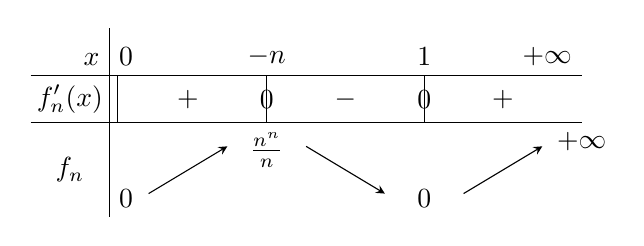
\begin{tikzpicture}[>=stealth,y=.6cm]
											\draw (-1,0) -- (6,0)
													(-1,-1) -- (6,-1)
 ;
											\draw (0,1) -- (0,-3)
													(0.1,0) -- (0.1,-1)
													(2,0) -- (2,-1)
													(4,0) -- (4,-1)
 ;
											\draw (0,0) node[above left] {$x$}
													(0,0) node[above right] {$0$}
													(2,0) node[above] {$\expo{-n}$}
													(4,0) node[above] {$1$}
													(6,0) node[above left] {$+\infty$}
 ;
											\draw (-.5 , -.5) node {$f'_n(x)$}
													(1,-.5) node {$+$}
													(2,-.5) node {$0$}
													(3,-.5) node {$-$}
													(4,-.5) node {$0$}
													(5,-.5) node {$+$}
 ;
											\draw (-.5,-2) node {$f_n$}
 ;
											\draw (0,-3) node[above right] {$0$};
											\draw[->] (0.5,-2.5) -- (1.5,-1.5);
											\draw (2,-1) node[below] {$\frac{n^n}{\expo{n}}$};
											\draw[->] (2.5,-1.5) -- (3.5,-2.5);
											\draw (4,-3) node[above] {$0$};
											\draw[->] (4.5,-2.5) -- (5.5,-1.5);
											\draw (6,-1) node[below] {$+\infty$};
										\end{tikzpicture}
									\end{figure}
									
									\vln{Tableau de variation de $f_2$ :}
										
									\begin{figure}[h!]
									\centering
										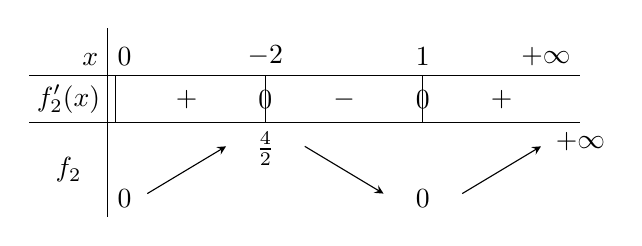
\begin{tikzpicture}[>=stealth,y=.6cm]
											\draw (-1,0) -- (6,0)
													(-1,-1) -- (6,-1)
 ;
											\draw (0,1) -- (0,-3)
													(0.1,0) -- (0.1,-1)
													(2,0) -- (2,-1)
													(4,0) -- (4,-1)
 ;
											\draw (0,0) node[above left] {$x$}
													(0,0) node[above right] {$0$}
													(2,0) node[above] {$\expo{-2}$}
													(4,0) node[above] {$1$}
													(6,0) node[above left] {$+\infty$}
 ;
											\draw (-.5 , -.5) node {$f'_2(x)$}
													(1,-.5) node {$+$}
													(2,-.5) node {$0$}
													(3,-.5) node {$-$}
													(4,-.5) node {$0$}
													(5,-.5) node {$+$}
 ;
											\draw (-.5,-2) node {$f_2$}
 ;
											\draw (0,-3) node[above right] {$0$};
											\draw[->] (0.5,-2.5) -- (1.5,-1.5);
											\draw (2,-1) node[below] {$\frac{4}{\expo{2}}$};
											\draw[->] (2.5,-1.5) -- (3.5,-2.5);
											\draw (4,-3) node[above] {$0$};
											\draw[->] (4.5,-2.5) -- (5.5,-1.5);
											\draw (6,-1) node[below] {$+\infty$};
										\end{tikzpicture}
									\end{figure}
							\end{enumerate}
						\item \vln{Positions relatives de $\CourbeD$ et $\CourbeT$ dans $]1 ; e[$ et dans $[e ; +\infty[$ :}
							\[
								f_3 (x) - f_2 (x) = x (\ln x)^3 - x (\ln x)^2 = x (\ln x)^2 (\ln x - 1)	.
							\]
							Comme $x > 0$ et $(\ln x)^2 \geq 0$, alors 
							le signe de $f_3(x) - f_2(x)$ est le m\^eme que celui de $(\ln x - 1)$.
							%
							\begin{figure}[h!]
							\centering
								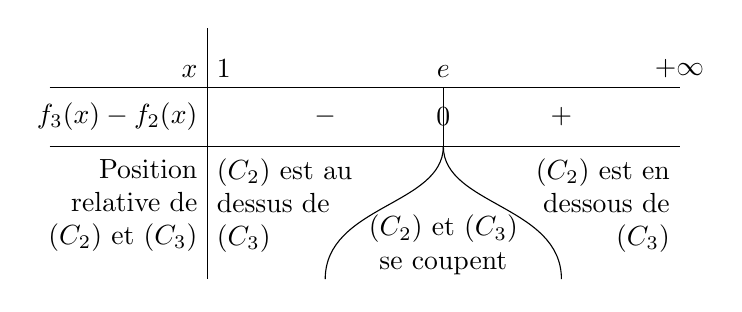
\begin{tikzpicture}[y=.75cm]
									\draw (-2,0) -- (6,0)
											(-2,-1) -- (6,-1)
 ;
									\draw (0,1) -- (0,-3.25)
											(3,0) -- (3,-1)
 ;
									\draw (3,-1) .. controls (3,-2) and (1.5,-2) .. (1.5,-3.25);
									\draw (3,-1) .. controls (3,-2) and (4.5,-2) .. (4.5,-3.25);
									\draw (0,0) node[above left] {$x$};
									\draw (0,0) node[above right] {$1$};
									\draw (3,0) node[above] {$e$};
									\draw (6,0) node[above] {$+\infty$};
									\draw (0,-.5) node[left] {$f_3(x)-f_2(x)$};
									\draw (1.5,-.5) node[] {$-$};
									\draw (3,-.5) node[] {$0$};
									\draw (4.5,-.5) node[] {$+$};
									\draw (0,-2) node[left] {\parbox{2cm}{\raggedleft Position relative de $\CourbeD$ et $\CourbeT$}};
									\draw (0,-2) node[right] {\parbox{2cm}{\raggedright $\CourbeD$ est au dessus de $\CourbeT$}};
									\draw (3,-2) node[below] {\parbox{2cm}{\centering $\CourbeD$ et $\CourbeT$ se coupent}};
									\draw (6,-2) node[left] {\parbox{2cm}{\raggedleft $\CourbeD$ est en dessous de $\CourbeT$}};
								\end{tikzpicture}
							\end{figure}
							%
							\begin{itemize}
								\item \ansbox{Sur $]1;e[$ : $\CourbeD$ est au dessus de $\CourbeT$.}
								\item \ansbox{$\CourbeD$ coupe $\CourbeT$ au point $(e,e)$.}
								\item \ansbox{Sur $[e;+\infty[$ : $\CourbeD$ est en dessous de $\CourbeT$.}
							\end{itemize}
						\item \vln{Montrons que le point $I(1,0)$ est un point d'inflexion de $\CourbeT$ :}\vspace{-1\baselineskip}
							\begin{align*}
								f_3 (x)	& = x \; (\ln x)^3 \\
								f'_3 (x)	& = [3+\ln x] \cdot [\ln x]^2 \\
								f''_3 (x)	& = \frac{1}{x} \cdot (\ln x)^2 + (3+\ln x) \cdot 2 \cdot \frac{1}{x} (\ln x) 	\\
											& = \frac{3 }{x} \cdot (\ln x) \cdot \left( \ln x + 2 \right)		.
							\end{align*}
							Pour tout $x>0$, $\frac{3}{x} > 0$ donc le signe de $f''_3(x)$ est le m\^eme que celui de 
							$\ln x \left( \ln x + 2 \right)$.
									\begin{figure}[H]
									\centering
										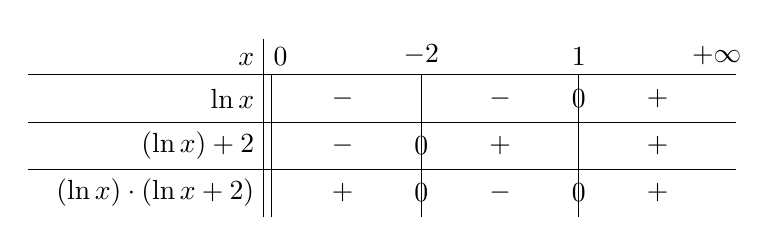
\begin{tikzpicture}[x=1cm,y=.6cm]
										\clip (-3,-3) rectangle (6.2,1);
											\draw (-3,0) -- (6,0) 
													(-3,-1) -- (6,-1) 
													(-3,-2) -- (6,-2) 
													(0,.75) -- (0,-3)
													(0.1,0) -- (0.1,-3)
													(2,0) -- (2,-3)
													(4,0) -- (4,-3);
											\draw (0,0) node[above left] {$x$}
													(0,0) node[above right] {$0$}
													(2,0) node[above] {$\expo{-2}$}
													(4,0) node[above] {$1$}
													(5.75,0) node[above] {$+\infty$};
											\draw (0,-.5) node[left] {$\ln x$}
													(1,-.5) node[] {$-$}
													(3,-.5) node[] {$-$}
													(4,-.5) node[] {$0$}
													(5,-.5) node[] {$+$};
											\draw (0,-1.5) node[left] {$(\ln x) + 2$}
													(1,-1.5) node[] {$-$}
													(2,-1.5) node[] {$0$}
													(3,-1.5) node[] {$+$}
													(5,-1.5) node[] {$+$};
											\draw (0,-2.5) node[left] {$(\ln x) \cdot (\ln x + 2)$}
													(1,-2.5) node[] {$+$}
													(2,-2.5) node[] {$0$}
													(3,-2.5) node[] {$-$}
													(4,-2.5) node[] {$0$}
													(5,-2.5) node[] {$+$};
										\end{tikzpicture}
									\end{figure}
									On constate que $f''_3$ s'annule en $1$ en changeant de signe ;
									on d\'eduit que
									\par\noindent\ansbox{le point $I(1,0)$ est un point d'inflexion de $\CourbeT$.}
									%
						\item \vln{Tra\c{c}age de $\CourbeD$ et $\CourbeT$ :}
								Voir Figure~\ref{fig: Bac 2004 Pbm II Representation graphique}.
							\begin{figure}
							\centering
								\begin{tikzpicture}[x=2cm,y=2cm]
									\Milimetre{(-.5,-1.5)}{(3.25,4.5)}
										\draw[color=black] (0,4.25) node [above left] {$y$};
										\draw[color=black] (3,0) node [above right] {$x$};
										\draw[->,color=black] (-0.5,0) -- (3.25,0);
										\foreach \x in {-1,1,2,3}
										\draw[shift={(\x,0)},color=black] (0pt,2pt) -- (0pt,-2pt) node[below] {\footnotesize $\x$};
										\draw[->,color=black] (0,-1.5) -- (0,4.5);
										\foreach \y in {-1,1,2,3,4}
										\draw[shift={(0,\y)},color=black] (2pt,0pt) -- (-2pt,0pt) node[left] {\footnotesize $\y$};
										\draw[color=black] (0,0) node[below left] {\footnotesize $O$};
										\draw [<->, >=stealth] (-0.08,0.54) -- (0.35,0.54);
										\draw [<->, >=stealth, loko1] (-0.17,-1.34) -- (0.27,-1.34);
										\draw [<->, >=stealth, brown, thick] (0.78,0) -- (1.22,0);
										\draw [dashed] (0.14,0.54)-- (0.14,0);
										\draw [dashed] (0.05,0)-- (0.05,-1.34);
										\draw [dashed] (0,2.72)-- (2.72,2.72);
										\draw [dashed] (2.72,2.72)-- (2.72,0);
										\draw [color=black,->] (0,0) -- (0,1);
										\draw[color=black] (0,0.75) node[left] {$\vec{\jmath}$};
										\draw [color=black,->] (0,0) -- (1,0);
										\draw[color=black] (0.75,0) node[below] {$\vec{\imath}$};
										\draw [color=loko2,->] (0,0) -- (0,.5);
										\draw [color=loko1,->] (0,0) -- (0,-.5);
										\draw[color=loko2, smooth,samples=250,domain={10^(-4)}:3.25] 
											plot(\x,{(\x)*ln((\x))^2});
										\draw[color=loko1, smooth,samples=250,domain={10^(-4)}:3.25] 
											plot(\x,{(\x)*ln((\x))^3});
										\begin{scriptsize}
%											\fill [color=black] (0.14,0) circle (1pt) node[below] {$\expo{-2}$};
											\fill [] (0.14,0.54) circle (1pt);
%											\fill [color=black] (0.05,0) circle (1pt) node[above] {$\expo{-3}$};
											\fill [color=black] (0.05,-1.34) circle (1pt);
											\fill [color=black] (1,0) circle (1pt);
											\fill [color=black] (2.72,2.72) circle (1pt);
											\fill [color=black] (0,2.72) circle (1pt) node[left] {$e$};
											\fill [color=black] (2.72,0) circle (1pt) node[below] {$e$};
										\end{scriptsize}
										\draw[color=loko2] (3,3.25) node[] {$\CourbeD$};
										\draw[color=loko1] (3,4) node[above left] {$\CourbeT$};
										% Ilay courbe-n'ilay fonction g (reciproque de la restriction de f_2 sur [1,e]).
										\draw[color=loko5b] (-1,-1) -- (4,4) 
											node [midway,sloped,below] {\textcolor{loko5b}{$y = x$}};
										\draw[color=loko3b, smooth,samples=250,domain=1:2.718] 
											plot({(\x)*ln((\x))^2},{\x});
										\draw[color=loko3b] (1.5,2.4) node {\rotatebox{22}{$y = g^{-1} (x)$}};
										\draw[color=loko3b,->] (0,1) -- (0,1.5);
								\end{tikzpicture}
								\caption{Courbes $\CourbeD$ de la fonction $f_2$ et $\CourbeT$ de la fonction $f_3$.}
								\label{fig: Bac 2004 Pbm II Representation graphique}
							\end{figure}
					\end{enumerate}
				\item[III. ]
					\begin{enumerate}
						\item \vln{Montrons que $g$ est une bijection :}
							La fonction $f_2$ est continue et strictement croissante sur $[1;+\infty[$.
							Par cons\'equent, $g$ est continue et strictement croissante ; elle r\'ealise donc une bijection
							de $[1,e]$ vers $g([1,e])=[0,e]$.
						\item \vln{Calcul $\left(g^{-1}\right)' (e)$ :}
							Comme $g(e) = e$ alors $g^{-1} (e) = e$.
							\begin{align*}
								\left(g^{-1}\right)' (e)	& = \frac{1}{g'\left( g^{-1} (e) \right)}			
																  = \frac{1}{g'(e)}										
																  = \frac{1}{f_2(e)}										
																  = \frac{1}{(2+\ln e) \cdot (\ln e)}				.
							\end{align*}
							Ainsi, \ansbox{$\left( g^{-1} \right)' (e) = \frac{1}{3}$}.
						\item \vln{Repr\'esentation graphique de $g^{-1}$ :}
								Voir Figure~\ref{fig: Bac 2004 Pbm II Representation graphique}.
					\end{enumerate}
			\end{description}
	\end{description}
%%%%%%%%%%%%%%%%%%%%%%%%%%%%%%%%%%%%%%%%%%%%%%%%%%%%%%%%%%%%%%%%%%%%%%%%%%%%%%%%%%%%%%%%%%%%%%%%%%%%%%%%%%%%%%%%%%%%%%%%%%%%%%%%



























